\section{IMPLEMENTATION DETAILS}
\subsection{Preprocessing}

Before training the model, we preprocess the dataset as follows:

\subsubsection{Resize}
All images, whether sourced from videos or other datasets, were resized to a consistent resolution of 256x256 pixels. This resizing ensured a uniform input size for the vision transformer.

\begin{figure}[ht]
    \centering
    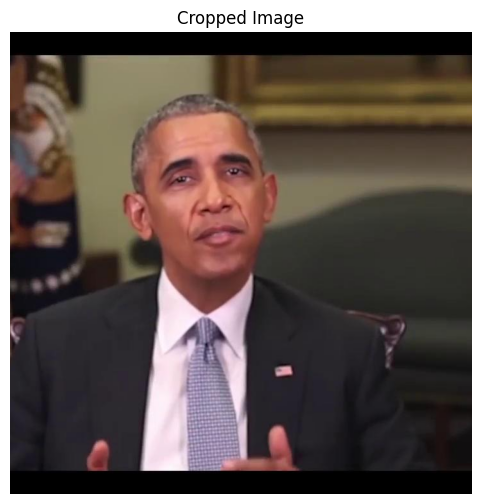
\includegraphics[width=2in]{img/cropped.png}
    \caption{Cropped Image}
    \label{fig:cropped}
\end{figure}

\begin{figure}[ht]
    \centering
    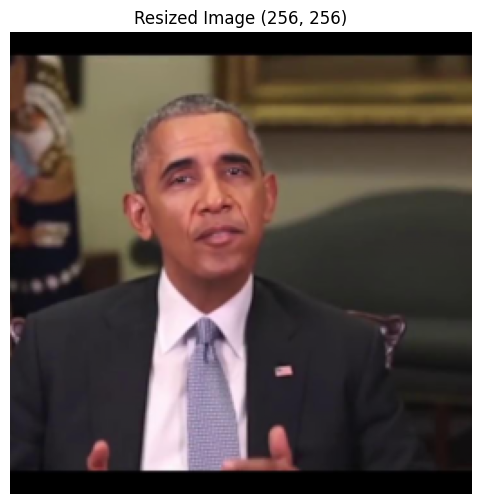
\includegraphics[width=2in]{img/resized.png}
    \caption{Resized Image}
    \label{fig:resized}
\end{figure}

% \subsubsection{Augmentation} To increase the dataset's diversity and improve the model's ability to generalize, we applied various data augmentation techniques. These techniques included random rotations, horizontal flips, brightness adjustments, and minor deformations.
% \newpage
\subsubsection{Normalization} Pixel values of the images were normalized to a specific range to ensure consistent input for the model during training and inference.

\begin{figure}[htbp]
    \centering
    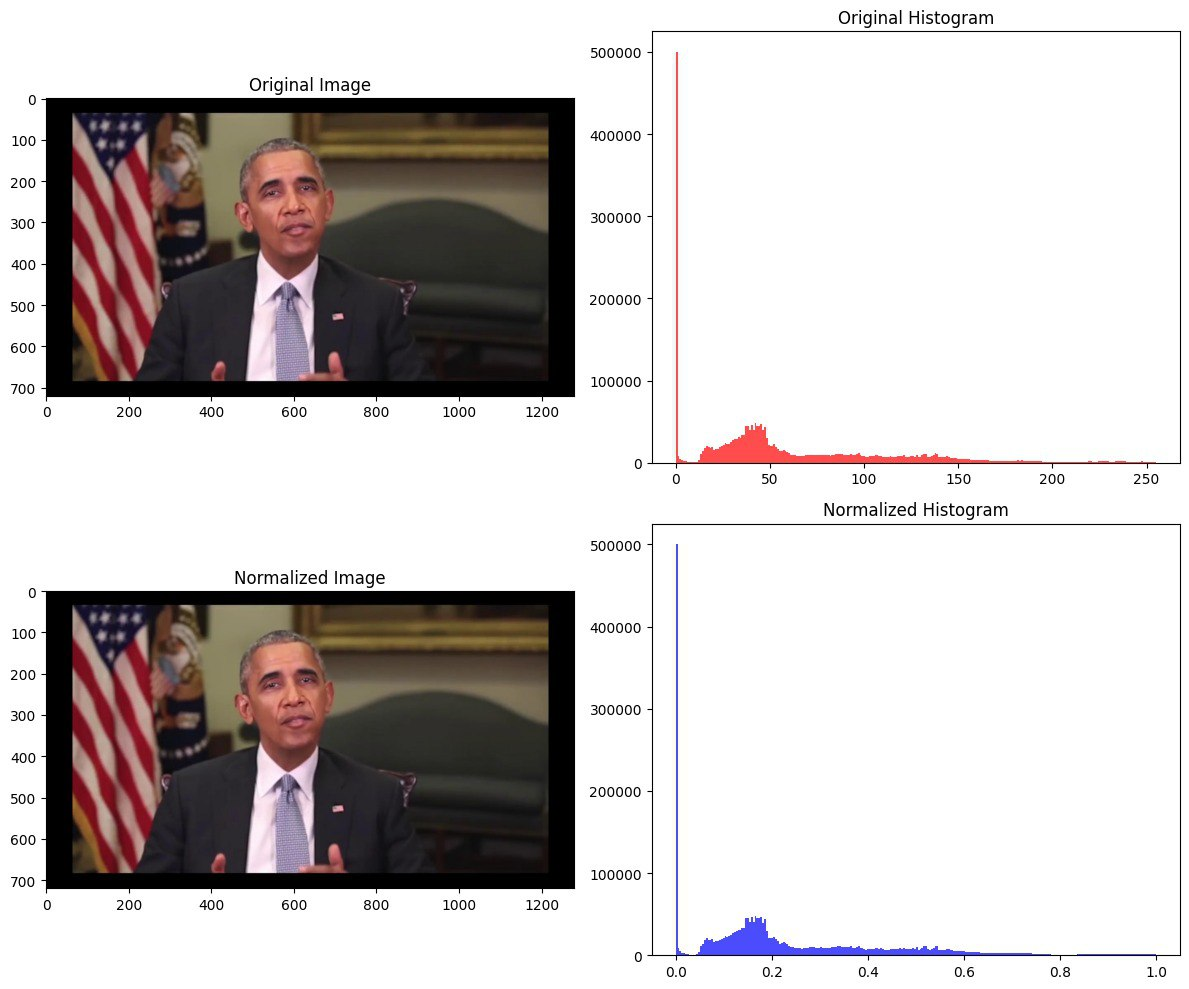
\includegraphics[width=5in]{img/normalized.jpg}
    \caption{Normalization}
\end{figure}

\noindent By preprocessing the dataset, we enhanced the model's capacity to learn relevant features and intricate patterns required for accurate deepfake detection.

\subsection{Face Alignment Integration}

The role of the Face Alignment library in the system is to contribute essential capabilities for precise face detection and facial feature extraction. The Face Alignment is the process of accurately aligning the facial landmarks (such as eyes, nose, and mouth) within an image to a canonical reference. This alignment is crucial for many tasks, including facial feature extraction, face recognition, and analysis of facial expressions. By integrating Face Alignment into our system, we are ensuring that the system can accurately detect faces, extract meaningful features, and analyze facial expressions with a high level of precision.

\subsubsection{Working Principle}

\begin{enumerate}
    \item \textbf{Landmark Detection:} The Face Alignment library employs advanced techniques to detect and locate key facial landmarks, such as the eyes, nose, and mouth. These landmarks serve as anchor points, enabling precise alignment and accurate feature extraction.

    \item \textbf{Face Localization:} This component utilizes dlib algorithms to identify and localize the face within an image. By determining the precise region of interest containing facial features, it enables focused analysis and enhances the overall accuracy of our system.

    \item \textbf{Affine Transformation:} Facial landmarks are aligned using affine transformation techniques. This transformation ensures a consistent and standardized positioning of features across different images. By achieving uniform alignment, we facilitate more accurate comparisons and enhance the robustness of our system against variations in facial expressions and poses.

\end{enumerate}

\begin{figure}[htbp]
    \centering
    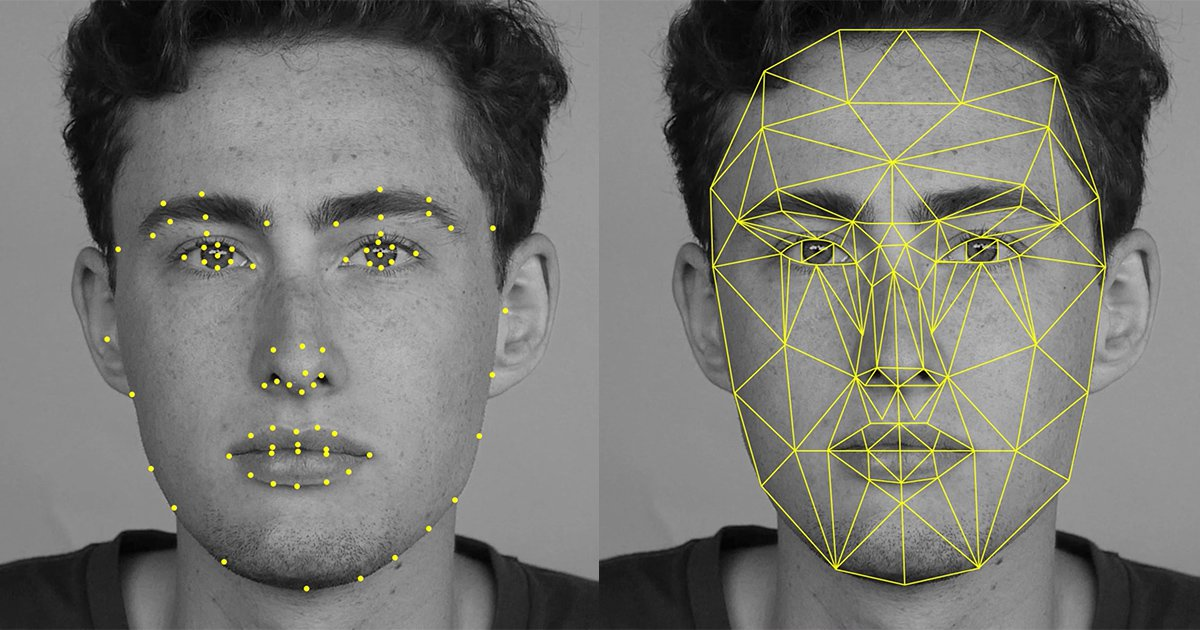
\includegraphics[width=5in]{img/facial feature.jpg}
    \caption{Facial Landmark Detection}
\end{figure}

\noindent By incorporating the Face Alignment library into our project, we ensure that facial features are consistently and accurately represented, thereby enhancing the overall performance of DefaceLab in detecting manipulated or fake media.\\